\chapter{Performance Analysis}
\label{cha:pa}

\lipsum[1]

\section{Time Performances}
\label{sec:pa_time}

\lipsum[1]

\begin{figure}[htbp]
  \centering
  \def\stackalignment{r}\stackunder{ 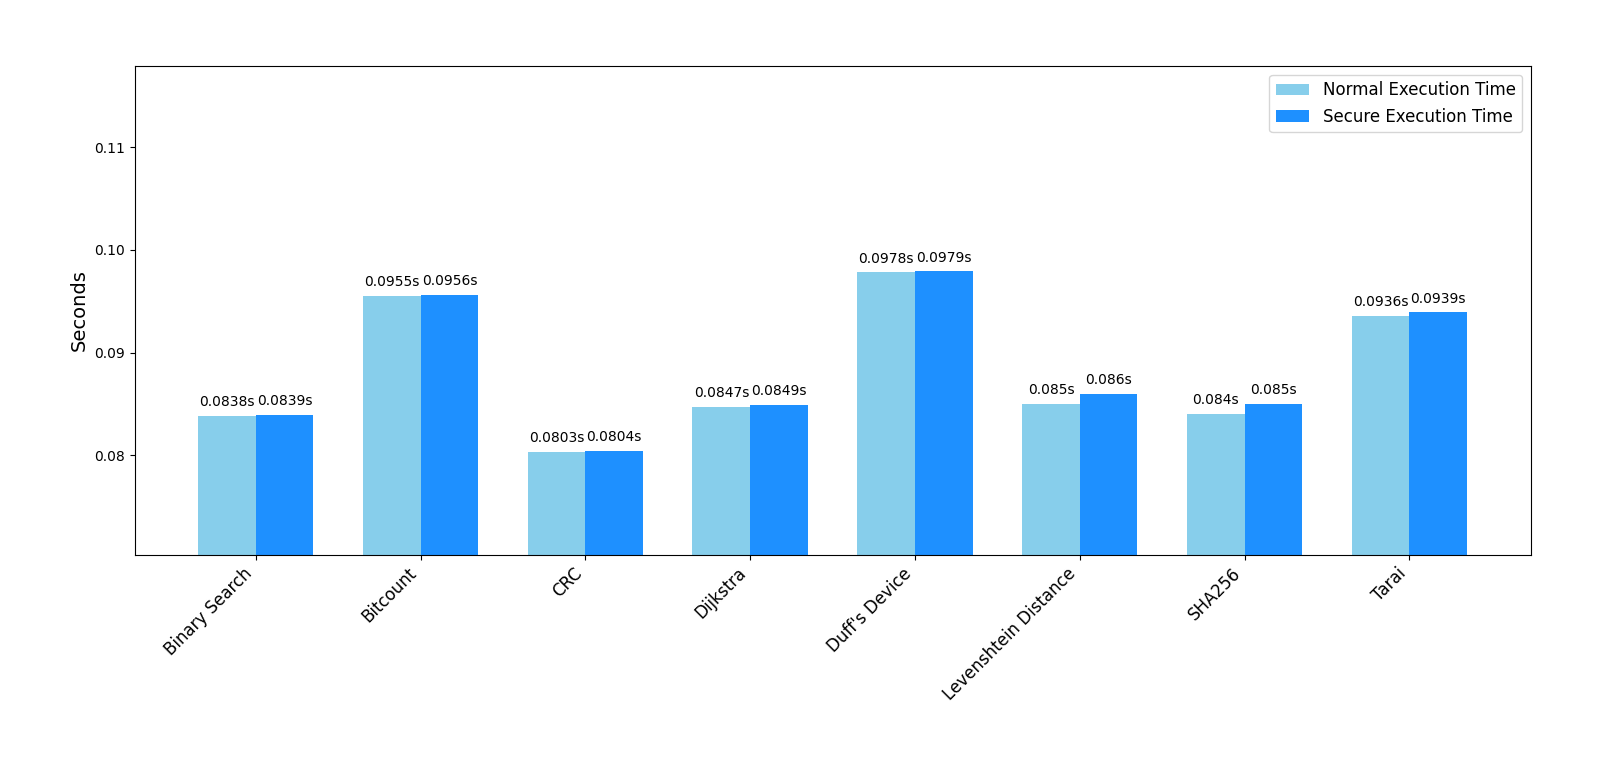
\includegraphics[width=.9\linewidth]{images/low_execution.png} } %
  {\scriptsize }
  \caption{Low execution times}
  \label{fig:lowtime}
\end{figure}

\begin{figure}[htbp]
  \centering
  \def\stackalignment{r}\stackunder{ 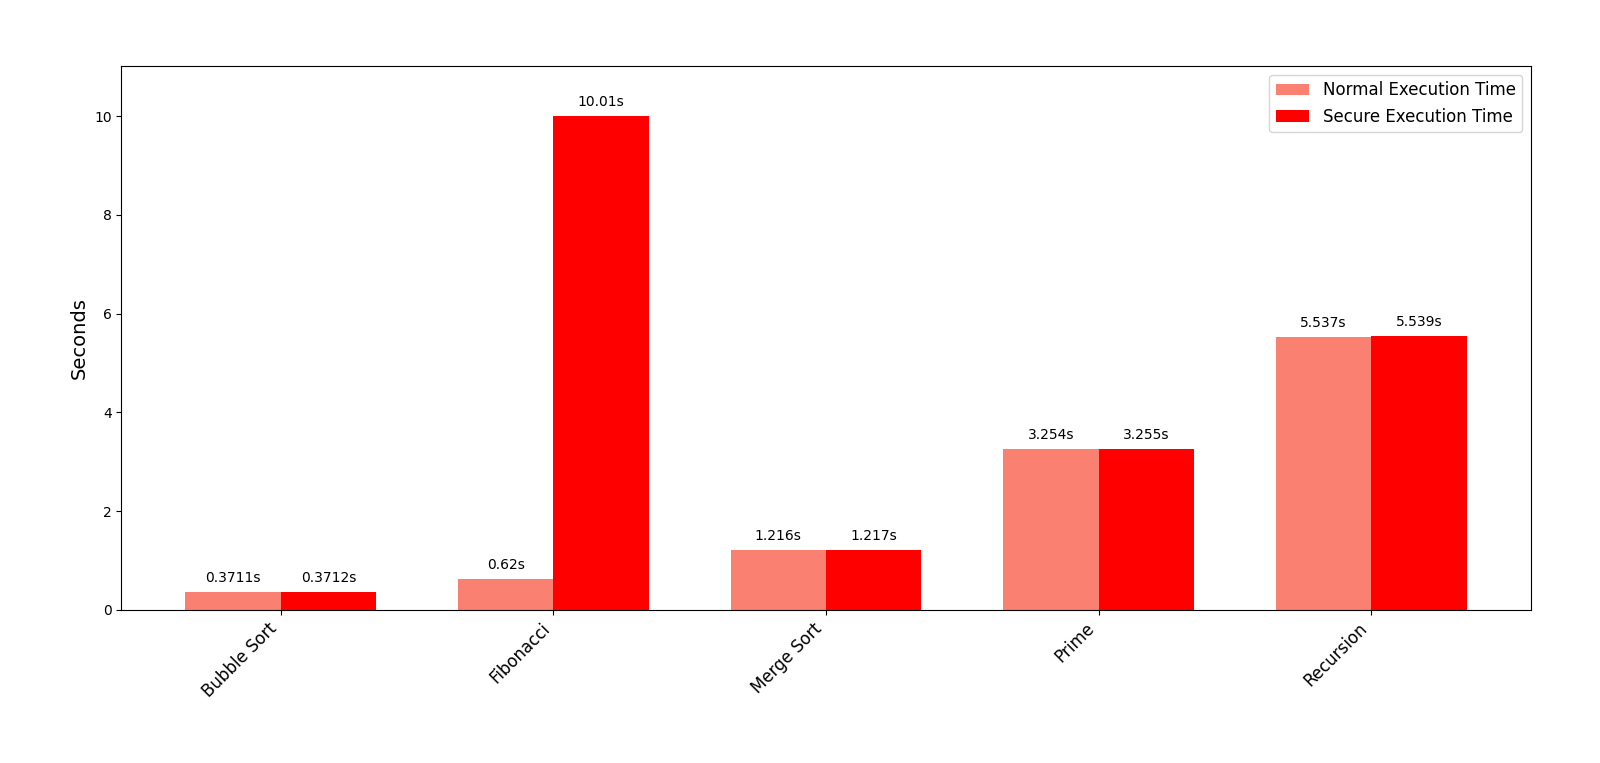
\includegraphics[width=.9\linewidth]{images/high_execution.png} } %
  {\scriptsize }
  \caption{High execution times}
  \label{fig:hightime}
\end{figure}

\begin{table}
  \centering
  \begin{tabular}{|c|c|c|c|}
    \hline
    \textbf{Algorithm}   & \textbf{Normal run time (s)} & \textbf{Secure run time (s)} & \textbf{Time Overhead} \\
    \hline
    Binary Search        & 0.08387                      & 0.08388                      & $0.012\%$              \\
    \hline
    Bitcount             & 0.0955                       & 0.0956                       & $0.11\%$               \\
    \hline
    Bubble Sort          & 0.37113                      & 0.37116                      & $0.008\%$              \\
    \hline
    CRC                  & 0.08025                      & 0.08026                      & $0.012\%$              \\
    \hline
    Dijkstra             & 0.0847                       & 0.0849                       & $0.236\%$              \\
    \hline
    Duff's Device        & 0.097795                     & 0.097799                     & $0.0041\%$             \\
    \hline
    Fibonacci            & 0.6166                       & 10.0089                      & $1523.24\%$            \\
    \hline
    Fibonacci Indirect   & 0.0849                       & 0.1511                       & $77.97\%$              \\
    \hline
    Levenshtein Distance & 0.085                        & 0.086                        & $1.176\%$              \\
    \hline
    Merge Sort           & 1.216                        & 1.217                        & $0.0822\%$             \\
    \hline
    Merge Sort Indirect  & 1.2168                       & 1.2169                       & $0.0082\%$             \\
    \hline
    Prime                & 3.254                        & 3.255                        & $0.03\%$               \\
    \hline
    Prime Indirect       & 3.253                        & 3.254                        & $0.03\%$               \\
    \hline
    Recursion            & 5.537                        & 5.539                        & $0.036\%$              \\
    \hline
    Recursion Indirect   & 5.537                        & 5.539                        & $0.036\%$              \\
    \hline
    SHA256               & 0.084                        & 0.085                        & $1.19\%$               \\
    \hline
    Tarai                & 0.0936                       & 0.0939                       & $0.32\%$               \\
    \hline
  \end{tabular}
  \caption{Comparison of execution times}
  \label{tab:times}
\end{table}

\begin{table}
  \centering
  \begin{tabular}{|c|c|c|c|}
    \hline
    \textbf{Algorithm}   & \textbf{Instrumentation (s)} & \textbf{Simulation (s)} & \textbf{CFG extraction (s)} \\
    \hline
    Binary Search        & 0.00296                      & no ind jumps            & 0.00174                     \\
    \hline
    Bitcount             & 0.00196                      & no ind jumps            & 0.00153                     \\
    \hline
    Bubble Sort          & 0.00302                      & no ind jumps            & 0.00175                     \\
    \hline
    CRC                  & 0.00203                      & no ind jumps            & 0.00154                     \\
    \hline
    Dijkstra             & 0.00264                      & no ind jumps            & 0.00182                     \\
    \hline
    Duff's Device        & 0.00265                      & no ind jumps            & 0.00163                     \\
    \hline
    Fibonacci            & 0.00209                      & no ind jumps            & 0.00149                     \\
    \hline
    Fibonacci Indirect   & 0.00202                      & 130.5567                & 0.07037                     \\
    \hline
    Levenshtein Distance & 0.00255                      & no ind jumps            & 0.00167                     \\
    \hline
    Merge Sort           & 0.00354                      & no ind jumps            & 0.00178                     \\
    \hline
    Merge Sort Indirect  & 0.0036                       & 4.6394                  & 0.00273                     \\
    \hline
    Prime                & 0.00214                      & no ind jumps            & 0.00168                     \\
    \hline
    Prime Indirect       & 0.00208                      & 11.4051                 & 0.00451                     \\
    \hline
    Recursion            & 0.00202                      & no ind jumps            & 0.00159                     \\
    \hline
    Recursion Indirect   & 0.00202                      & 23.2751                 & 0.00875                     \\
    \hline
    SHA256               & 0.00411                      & no ind jumps            & 0.00189                     \\
    \hline
    Tarai                & 0.00198                      & no ind jumps            & 0.00152                     \\
    \hline
  \end{tabular}
  \caption{Comparison of execution times}
  \label{tab:othertimes}
\end{table}

\section{Memory Overhead}
\label{sec:pa_memory}

\lipsum[1]

\begin{figure}[htbp]
  \centering
  \def\stackalignment{r}\stackunder{ 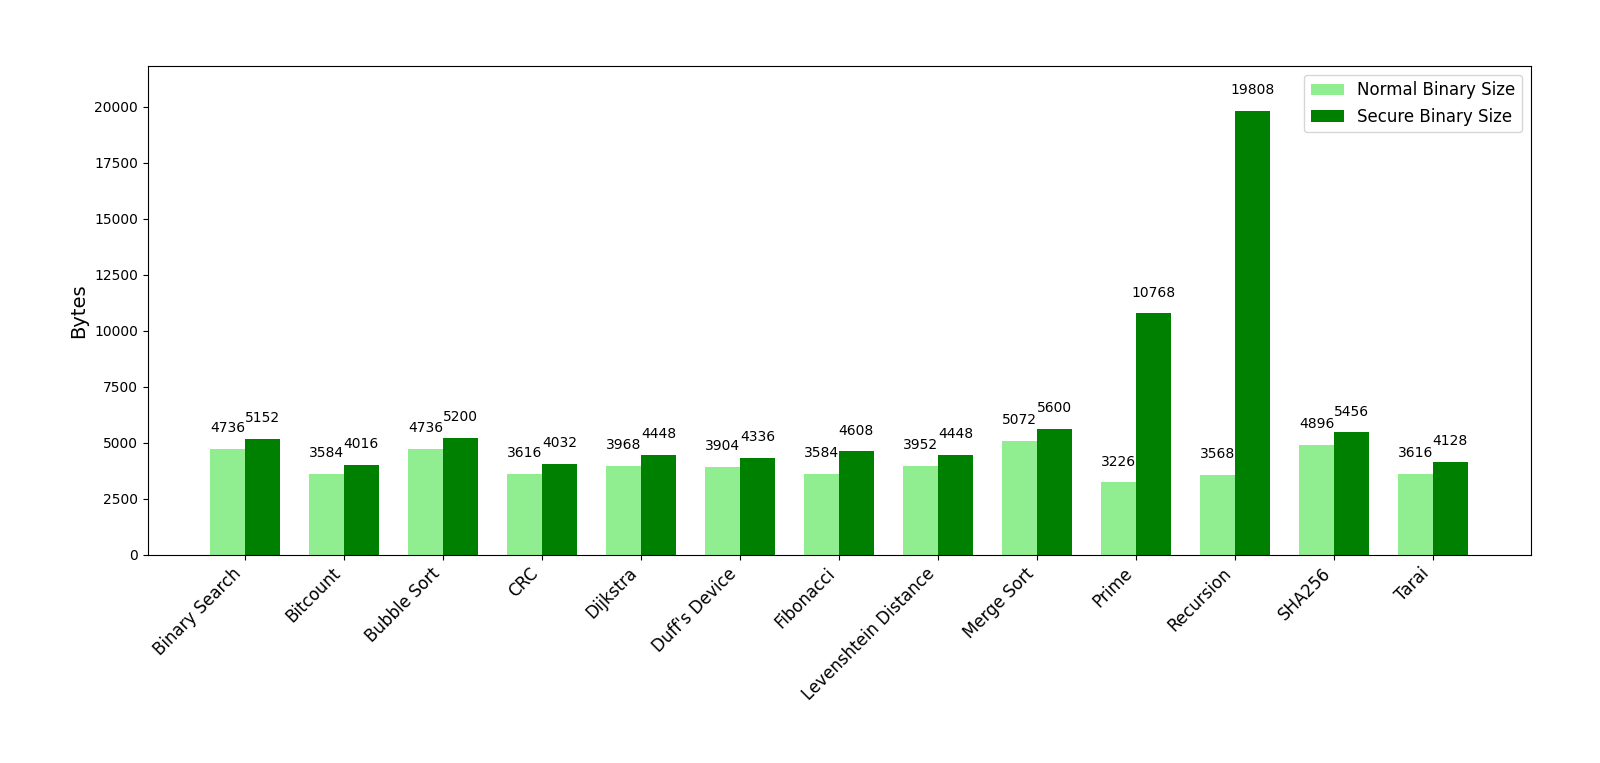
\includegraphics[width=.9\linewidth]{images/bin_sizes.png} } %
  {\scriptsize }
  \caption{Binary sizes}
  \label{fig:binsize}
\end{figure}

\begin{table}
  \centering
  \begin{tabular}{|c|c|c|c|}
    \hline
    \textbf{Algorithm}   & \textbf{Normal bin size (B)} & \textbf{Secure bin size (B)} & \textbf{Memory Overhead} \\
    \hline
    Binary Search        & 4736                         & 5152                         & $8.78\%$                 \\
    \hline
    Bitcount             & 3584                         & 4016                         & $12.05\%$                \\
    \hline
    Bubble Sort          & 4736                         & 5200                         & $9.79\%$                 \\
    \hline
    CRC                  & 3616                         & 4032                         & $11.51\%$                \\
    \hline
    Dijkstra             & 3968                         & 4448                         & $12.09\%$                \\
    \hline
    Duff's Device        & 3904                         & 4336                         & $11.06\%$                \\
    \hline
    Fibonacci            & 3584                         & 4608                         & $28.57\%$                \\
    \hline
    Fibonacci Indirect   & 3600                         & 4064                         & $12.88\%$                \\
    \hline
    Levenshtein Distance & 3952                         & 4448                         & $12.55\%$                \\
    \hline
    Merge Sort           & 5072                         & 5600                         & $10.41\%$                \\
    \hline
    Merge Sort Indirect  & 5088                         & 5600                         & $10.06\%$                \\
    \hline
    Prime                & 3226                         & 10768                        & $233.78\%$               \\
    \hline
    Prime Indirect       & 3712                         & 10768                        & $190.08\%$               \\
    \hline
    Recursion            & 3568                         & 19808                        & $455.15\%$               \\
    \hline
    Recursion Indirect   & 3584                         & 19808                        & $452.68\%$               \\
    \hline
    SHA256               & 4896                         & 5456                         & $11.43\%$                \\
    \hline
    Tarai                & 3616                         & 4128                         & $14.16\%$                \\
    \hline
  \end{tabular}
  \caption{Comparison of binary sizes}
  \label{tab:binsize}
\end{table}

\section{Optimization Techniques}
\label{sec:pa_optimization}

\lipsum[1]

\section{Results and Analysis}
\label{sec:pa_results}

\lipsum[1]